\documentclass[twocolumn]{article}
\usepackage[a4paper, top=1in, bottom=1in, left=2cm, right=2cm]{geometry}
\usepackage[singlespacing]{setspace}
\usepackage{amsmath}
\usepackage{amssymb}
\usepackage{graphicx}
\usepackage{hyperref}
\title{Rediscovery of astroid from the refraction image by a flat boundary}
\author{M. Ryu \\ {\href{mailto:mingshey@hafs.hs.kr}{mingshey@hafs.hs.kr}}}
\begin{document}
\maketitle
\section{Introduction}
The phenomenon of a pencil appearing bent when partly submerged in water is a 
familiar sight commonly encountered when first learning about refraction. 
However, it is observable that the tip of the pencil does not always appear 
at the same location. While the depth when viewed directly from above is 
covered in introductory physics courses, the reasons behind the variations 
in depth and apparent position when viewed obliquely often remain unexplored. 
Perhaps it is considered too complex to delve into in depth. In fact, in 
advanced optics textbooks, this simple question is often overlooked in favor 
of more significant topics such as lenses and mirrors.

Nevertheless, this seemingly simple yet intriguing question continues to 
pique our curiosity. It is likely that others, besides the author, have 
pondered this question. This study aims to provide an answer.

\section{Quick Answer}
For the impatient reader, here's the quick answer:
Consider a point object submerged in water. The observation point (POV) is 
located above the water surface. The object and the POV lie within a common normal plane. 

Let the normal plane that contains the object and  POV be the $xy$-plane,
and let the intersection of  normal plane and the surface of water be the 
$x$-axis, and the normal through  object $y$-axis.

As the POV moves within the normal plane, the apparent position of the 
object changes. The locus of these apparent positions forms a curve, 
which can be classified as a type of caustic\footnote{Since this is a 
locus of virtual images, it can be termed a \emph{virtual caustic}.}. 

It is shown that this caustic curve is a \emph{squashed astroid}
and can be described by the following equation:

$$ \left| \dfrac{x}{M} \right| ^ {2/3} + \left| \dfrac{y}{N} \right| ^ {2/3} = 1,$$
where 
$M = D/\sqrt{n^2 - 1}$ represents the maximum distance of incidence determined 
by the critical angle of total internal reflection, 
$N = D/n$ represents the apparent depth of the object when observed directly 
from above,
$D$ is the actual depth of the object, and
$n$ is the refractive index of water relative to air.

\begin{figure}[htbp]
	\centering
	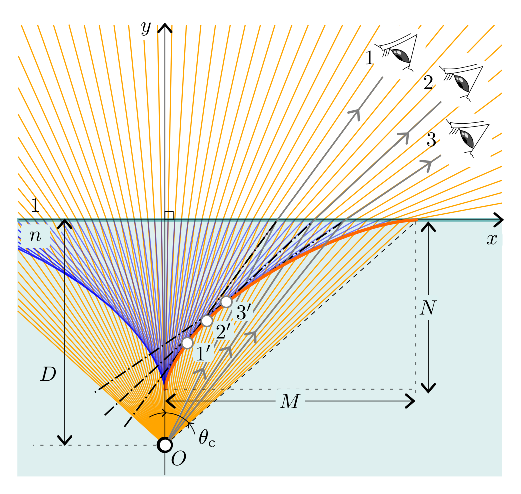
\includegraphics[width=2.7in]{g409.eps}
	\caption{Illustration of the caustic curve formed by the apparent positions of a submerged object as viewed from above the water surface.}
	\label{fig:caustic_curve}
\end{figure}

\section{Derivation of the Formula}

Consider a point object O submerged at a depth D below the planar interface 
between air (refractive index $n_1$) and water (refractive index $n_2$). 
A ray of light emanating from O strikes the interface at point A, located a 
distance $\alpha$ from the y-axis. The incident ray makes an angle $\theta_2$ 
with the normal at A, and the refracted ray in air makes an angle $\theta_1$ 
with the same normal.

From Snell's law we have
$$ \sin\theta_1 = \frac{n_2}{n_1} \sin\theta_2 = n\sin\theta_2.$$
The extension of refracted ray is described by the equation 
$$y=k(x-\alpha),$$
where 
$$k=\dfrac{1}{\tan\theta_1}=\dfrac{\cos\theta_1}{\sin\theta_1},$$
and considering the Snell's law,
$$k=\dfrac{\sqrt{1-n^2\sin^2\theta_2}}{n\sin\theta_2}.$$

\begin{figure}[htbp]
	\centering
	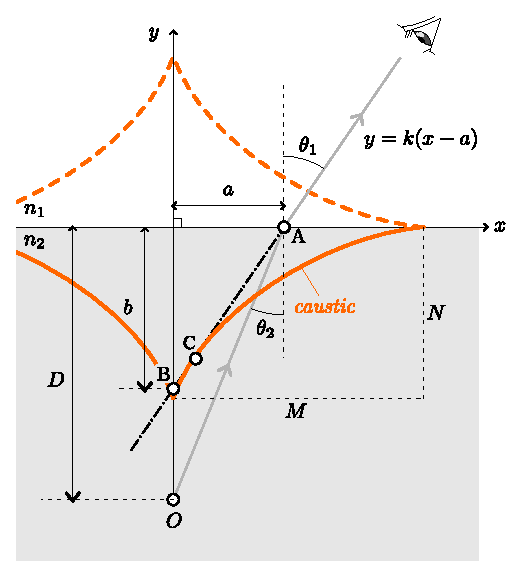
\includegraphics[width=3in]{g237.eps}
	\caption{Geometry of light refraction at the air-water interface.} 
\end{figure}

This line meets the $y$-axis at B($y=\beta$), thus
$$\beta = -k\alpha.$$

By the geometry we have
$$\alpha = D\tan\theta_2 = \dfrac{D\sin\theta_2}{\cos\theta_2},$$
and
$$\begin{aligned}
	\beta &= -k\alpha \\
	&= -\dfrac{D\sin\theta_2}{\cos\theta_2}
	\dfrac{\sqrt{1-n^2\sin^2\theta_2}}{n\sin\theta_2}\\
	&=-\dfrac{D\sqrt{1-n^2\sin^2\theta_2}}{n\cos\theta_2}.
\end{aligned}$$
Now, let $K=\alpha/M$ and $H=\beta/N$, then
$$ \begin{aligned}
	K^2 + H^2 &= \dfrac{\alpha^2}{M^2}+\dfrac{\beta^2}{N^2}\\
	&=\dfrac{\left(n^2-1\right)\sin^2\theta_2 + 1-n^2\sin^2\theta_2}
	{\cos^2\theta_2}\\
	&=\dfrac{1-\sin^2\theta_2}{\cos^2\theta_2}\\
	&=1
\end{aligned}$$

We introduce dimensionless parameters $\xi=x/M$ and $\eta=y/N$. 
As the POV traverses the $xy$-plane, the corresponding points transform accordingly:
Point $\mathrm{A}(\alpha, 0)$ in object space maps to $\mathrm{K}(K, 0)$ in the $\xi\eta$-plane 
and point $\mathrm{B}(0, \beta)$ in object space maps to $\mathrm{H}(0, H)$ in the $\xi\eta$-plane. 
Crucially, the distance between these transformed points remains constant and equal 
to unity throughout the movement of the POV.

\begin{figure}[htbp]
	\centering
	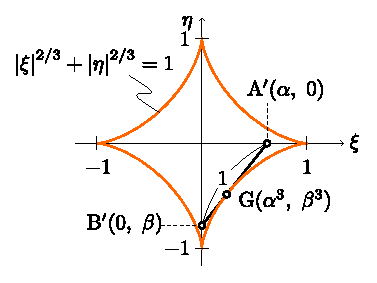
\includegraphics{g107.eps}
	\caption{Geometric representation in the transformed $\xi\eta$-plane.} 
\end{figure}

The locus of the segment $\overline{\mathrm{KH}}$ in the $\xi\eta$-plane, generates an envelope, which is a 
well-defined geometric shape known as an astroid (not to be confused with an asteroid). 
Mathematically, an astroid is described by the following equation:

$$ \left| \xi \right|^{2/3} + \left| \eta \right|^{2/3} = 1 $$

The image of the submerged object is located at the point of tangency (point $\mathrm{C}$) 
between the segment $\overline{\mathrm{AB}}$(in object space) and the caustic. 
This tangency point signifies the point of divergence for the 
neighboring bundle of light rays. The corresponding coordinates of point $\xi\eta$-plane is 
$\mathrm{G}(K^3, H^3)$.

Thus we can obtain the coordinates of image $(x_{\mathrm{C}}^{}, y_{\mathrm{C}}^{})$ 
from the relation
$$ \left\{ 
\begin{aligned}
	\xi_{\mathrm{G}}^{} &= \dfrac{x_{\mathrm{C}}^{}}{M} = K^3 = \dfrac{\alpha^3}{M^3},\\
	\eta_{\mathrm{G}}^{} &= \dfrac{y_{\mathrm{C}}^{}}{N} = H^3 = \dfrac{\beta^3}{N^3}.
\end{aligned}
\right.$$

That is
$$ \left\{ 
\begin{aligned}
	x_{\mathrm{C}}^{} &= \dfrac{\alpha^3}{M^2},\\
	y_{\mathrm{C}}^{} &= \dfrac{\beta^3}{N^2}=-\dfrac{k^3\alpha^3}{N^2}.
\end{aligned}
\right.$$

Using 
$$\sin\theta_2 = \dfrac{\alpha}{\sqrt{D^2+\alpha^2}},$$
we have
$$k = \dfrac{\sqrt{D^2-(n^2-1)\alpha^2}}{n\alpha},$$
and we can derive the position of the image as parametric functions w.r.t. $\alpha$:
$$ \left\{ 
\begin{aligned}
	x_{\mathrm{C}}^{} &= (n^2-1)\dfrac{\alpha^3}{D^2},\\
	y_{\mathrm{C}}^{} &= -\dfrac{n^2}{D^2}\dfrac{\alpha^3}{n^3\alpha^3}\left\{ D^2-(n^2-1)\alpha^2 \right\}^{3/2}\\
	&=-\dfrac{D}{n}\left\{ 1-(n^2-1)\dfrac{\alpha^2}{D^2} \right\}^{3/2}.
\end{aligned}
\right.$$

\section{Underwater Viewpoint}

Consider an object positioned at a height $D$ above a flat interface separating air and water. If the  POV is submerged in water, the relative refractive index becomes less than one, expressed as $1/n < 1$. Following similar reasoning, we can derive the equation for the caustic as:

$$ \left| \xi \right|^{2/3} - \left| \eta \right|^{2/3} = -1, $$

where $\xi = \dfrac{x}{W}$, $\eta = \dfrac{y}{Z}$, $W = \dfrac{nD}{\sqrt{n^2-1}}$, and $Z = nD$. This curve exhibits asymptotes with slopes of $\pm Z/W = \pm \sqrt{n^2-1}$.

Consequently, the observed image of the \emph{skyscape} above the water, as seen from underwater, is compressed into a circular region (or more precisely, a cone) bounded by the critical angle of total internal reflection, known as Snell's window. This wide-angle, circular view perceived by an underwater observer resembles the field of view captured by a fisheye lens.

A specific name for this caustic curve shape appears to be absent in the current literature. The generalized form of this curve,

$$ \left| \xi \right|^{2/3} - \left| \eta \right|^{2/3} = \pm1, $$
%
holds physical significance as the caustic of rays emanating from a point light source above water and refracted into water. Given this significance and its relationship to the astroid, analogous to the connection between a hyperbola and an ellipse, we propose the term \emph{hyperastroid} as a suitable nomenclature.

\begin{figure}[h]
	\centering
	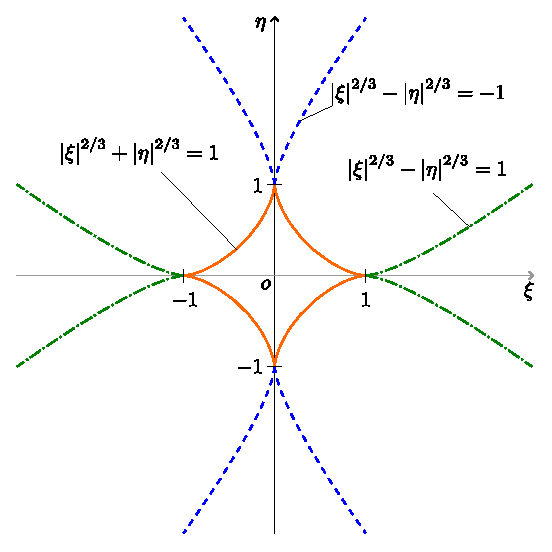
\includegraphics[width=3in]{g254.eps}
	\caption{An astroid and its hyperbolic counterparts}
	\label{fig:caustic}
\end{figure}

The astroid belongs to the family of curves known as \emph{superellipses} (see \href{https://mathworld.wolfram.com/Astroid.html}{MathWorld}), defined by the equation:

$$ \left| \xi \right|^{r} + \left| \eta \right|^{r} = 1. $$
%
An astroid is the special case where $r=2/3$. 

A similar family of curves, defined by
$$
\left| \xi \right|^{r} - \left| \eta \right|^{r} = \pm 1,
$$
%
has been called \emph{super hyperbolas} in \href{http://dynamicmathematicslearning.com/super-ellipse.html}{DML} \footnote{\ttfamily{dynamicmathematicslearning.com/super-ellipse.html}}. A collective term \emph{superconics} is used in \href{https://old.nationalcurvebank.org/superconicncb/superconicncb.htm}{NCB} \footnote{\ttfamily{nationalcurvebank.org/superconicncb/superconicncb.htm}}, but I have not found other instances of these terms in the literature and am uncertain if they are established terms in the field.

\section{Locating of the Image}

The closed-form solution of the caustic curve allows us to analytically determine the image location for a given object and point of view (POV).

\begin{figure}[htbp]
	\centering
	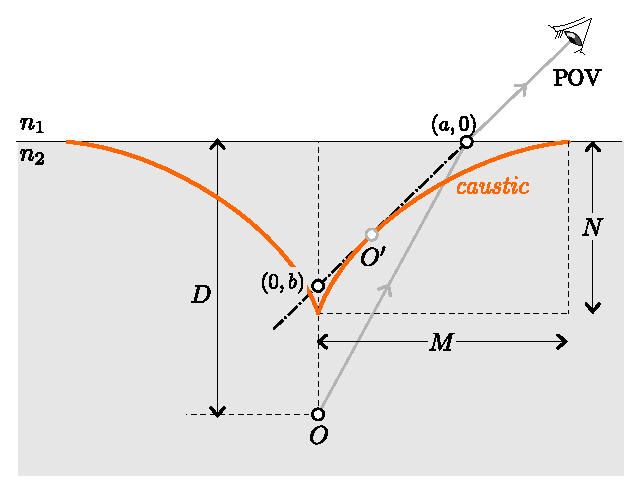
\includegraphics[width=3in]{g394.eps}
	\caption{Finding the image location using the caustic curve. The tangent line from the POV (dot and dash) intersects the caustic (orange) at the image point ($O^\prime$). The intersection with the water surface marks the light ray incidence point. }
	\label{fig:image_location}
\end{figure}

A tangent line is drawn from the POV to the caustic curve. The point of tangency between this line and the caustic represents the image location of the point source. Simultaneously, the intersection point of the tangent line with the water surface identifies the point of incidence for the light ray originating from the object.

For an extended object submerged in water, the image of each point on its surface can be determined using the same procedure. The collection of these individual image points, as each point traverses the object's surface continuously, forms the image of the extended object.

\begin{figure}[htbp]
	\centering
	\includegraphics*[width=3in]{g240.eps}
	\caption{Image formation for an extended object. Light rays from each point on the object (solid blue line) travel through water and refract, forming the image (dashed curve).}
	\label{fig:extended_object}
\end{figure}

However, analytically finding the tangent line to the caustic can be challenging, if not impossible. In practice, we resort to numerical methods to obtain an approximate solution.

An alternative approach involves numerically tracing the light ray path connecting the object and the viewpoint using Fermat's principle. Then, based on the coordinates of the light ray's intersection point with the water surface, the tangent point formula of the astroid can be used to locate the image. A Python implementation for this method can be found at \href{https://github.com/mingshey/python_projects/blob/main/Refraction_Image_en.ipynb}{github.com/mingshey/python\_projects}.

\appendix
\newcommand{\pd}[2]{\frac{\partial #1}{\partial #2}} % Simplified command for partial derivative
\newcommand{\ilpd}[2]{{\partial #1}/{\partial #2}}
\section*{The Astroid as an Envelope}

Consider two points in the Cartesian plane: $(K, 0)$ on the x-axis and $(0, H)$ on the y-axis, moving such that the distance between them remains constant, denoted by $a$. This constraint implies $K^2 + H^2 = a^2$. 

The equation of the line segment connecting these points at any given instant can be expressed as:

\begin{equation*}
	y = -\frac{H}{K}(x-K)
\end{equation*}

Substituting $H = \pm \sqrt{a^2 - K^2}$ yields:

\begin{equation*}
	y(x, K) = \mp \frac{\sqrt{a^2 - K^2}}{K}(x-K)
\end{equation*}

As the value of $K$ varies, the line segment connecting the two points also changes. The envelope of this family of lines is defined as the locus of points that are stationary with respect to infinitesimal variations in $K$, i.e., the points where $\ilpd{y}{K} = 0$. 

To determine the coordinates of these stationary points, we differentiate $y(x, K)$ with respect to $K$:

\begin{align*}
	\pd{y}{K} &= \pm \left[ \left( \frac{1}{\sqrt{a^2 - K^2}} + \frac{\sqrt{a^2 - K^2}}{K^2} \right)(x-K) + \frac{\sqrt{a^2 - K^2}}{K} \right] \\
	&= \pm \frac{(K^2 + a^2 - K^2)(x-K) + K(a^2 - K^2)}{K^2 \sqrt{a^2 - K^2}} \\
	&= \pm \frac{a^2 x - K^3}{K^2 \sqrt{a^2 - K^2}} \\
	&= 0. 
\end{align*}

Therefore, the abscissa of the stationary point is given by $x = K^3/a^2$. 

The corresponding ordinate can be found by substituting this value of $x$ back into the equation for $y(x, K)$:

\begin{align*}
	y(x, K) &= \mp \frac{\sqrt{a^2 - K^2}}{K} \left( \frac{K^3}{a^2} - K \right) \\
	&= \pm \frac{(a^2 - K^2)^{3/2}}{a^2} \\
	&= \frac{H^3}{a^2}
\end{align*}

Consequently, the coordinates $(x, y)$ of the stationary points satisfy the following equation:

\begin{equation*}
	\left| \frac{x}{a} \right|^{2/3} + \left| \frac{y}{a} \right|^{2/3} = 1.
\end{equation*}
$\blacksquare$


\end{document}

